\documentclass{UTNetLab}

\title{Network Management and Security}
\newcommand\reference{
   S. Panwar, S. Mao, J.-dong Ryoo, and Y. Li, “Network management and security,” in TCP/IP Essentials: A Lab-Based Approach, Cambridge: Cambridge University Press, 2004, pp. 187–213.
}
\newcommand{\difficultyscore}{6/10}     % modified UTNetLab.cls

\newcommand{\host}[1]{h\textsubscript{#1}'s Console}
\newcommand{\auxhost}[1]{h\textsubscript{#1}'s Auxiliary Console}
\newcommand{\termlbl}[2][red!10]{\fcolorbox{blue}{#1}{#2}}
\newcommand{\auxlbl}[2][blue!10]{\fcolorbox{blue}{#1}{#2}}
\newcommand{\guilbl}[2][green!10]{\fcolorbox{blue}{#1}{#2}}
\newcommand{\caplbl}[2][blue!10]{\fcolorbox{black}{#1}{#2}}
\newcommand{\filelbl}[3][black!5]{\fcolorbox{gray}{#1}{#2\texttt{:}#3}}
\newcommand{\lstsetterm}{\lstset{backgroundcolor=\color{red!10}}}
\newcommand{\lstsetaux}{\lstset{backgroundcolor=\color{blue!10}}}
\newcommand{\lstsetgui}{\lstset{backgroundcolor=\color{green!10}}}
\newcommand{\lstsetfile}{\lstset{backgroundcolor=\color{black!5}}}

% TODO: hX.netlab as hostnames

\begin{document}
	\section*{Objectives}
	\begin{itemize}
		\item SNMP and MIBs, using NET-SNMP as an example, and using NETSNMP utilities to query MIB objects.
		\item Encryption, confidentiality, and authentication, including DES, AES, RSA, MD5 and DSS.
		\item Application layer security, using SSH and Kerberos as examples.
		\item Transport layer security, including SSL and the secure Apache server.
		\item Network layer security, IPsec and Virtual Private Networks.
		\item Firewalls and IPTABLES.
		\item Accounting, auditing, and intrusion detection.
	\end{itemize}
\part{SNMP Exercises}
    For exercises 1-7 in this laboratory manual, the network topology is given in \hyperref[fig:1.3]{Figure~1.3}, where all the hosts are connected in a single network segment using their IP addresses, i.e.\  from 128.238.66.100 to 128.238.66.107.

    \begin{center}
        \begin{minipage}{0.48\textwidth}
            \begin{flushleft}
                \begin{table}[H]
                    \caption{The IP addresses of the hosts (Table~1.2)}
                    \centering
                    \begin{tabular}{ c c c }
                        \hline \hline
                        Host & IP Address & Subnet Mask \\
                        \hline 
                        h0 & 128.238.66.100 & 255.255.255.0 \\
                        h1 & 128.238.66.101 & 255.255.255.0 \\
                        h2 & 128.238.66.102 & 255.255.255.0 \\
                        h3 & 128.238.66.103 & 255.255.255.0 \\
                        h4 & 128.238.66.104 & 255.255.255.0 \\
                        h5 & 128.238.66.105 & 255.255.255.0 \\
                        h6 & 128.238.66.106 & 255.255.255.0 \\
                        h7 & 128.238.66.107 & 255.255.255.0 \\
                        \hline \hline
                        \end{tabular}
                \end{table}
            \end{flushleft}
        \end{minipage}
        \begin{minipage}{0.48\textwidth}
            \begin{flushright}
                \begin{figure}[H]
                    \centering
                    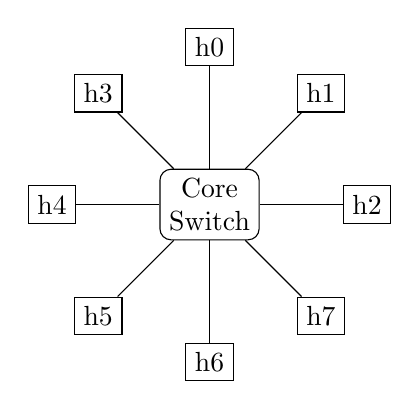
\begin{tikzpicture}
                        \node[draw,align=center,rounded corners] (s) at (0,0){Core\\Switch};
                        \node[draw] (h0) at (0,2){h0};
                        \node[draw] (h1) at ({sqrt(2)},{sqrt(2)}){h1};
                        \node[draw] (h2) at (2,0){h2};
                        \node[draw] (h3) at (-{sqrt(2)},{sqrt(2)}){h3};
                        \node[draw] (h4) at (-2,0){h4};
                        \node[draw] (h5) at (-{sqrt(2)},-{sqrt(2)}){h5};
                        \node[draw] (h6) at (0,-2){h6};
                        \node[draw] (h7) at ({sqrt(2)},-{sqrt(2)}){h7};
                    
                        \draw (h0) -- (s);
                        \draw (h1) -- (s);
                        \draw (h2) -- (s);
                        \draw (h3) -- (s);
                        \draw (h4) -- (s);
                        \draw (h5) -- (s);
                        \draw (h6) -- (s);
                        \draw (h7) -- (s);
                    \end{tikzpicture}
                    \caption{A single segment network (Figure~1.3)}\label{fig:1.3}
                \end{figure}
            \end{flushright}
        \end{minipage}
    \end{center}

\section{SNMP Service and MIB Struct}
    Before the lab, you should do these instructions on \textit{\host{0}}:
    \begin{enumerate}
        \item Backup the original \lstinline{snmpd} configuration file:
        
        \termlbl{\host{0}}
        \lstsetterm
        \begin{lstlisting}
    mv /etc/snmp/snmpd.conf /etc/snmp/snmpd.conf.save
        \end{lstlisting}
        \item Create a simple configuration file \path{/etc/snmp/snmpd.conf}  containing a single line defining a read-only community \textbf{guest}:
        
        \termlbl{\host{0}}
        \lstsetterm
        \begin{lstlisting}
    nano /etc/snmp/snmpd.conf
    # after opening the file, write this inside it:
    rocommunity guest
        \end{lstlisting}                
    
    Save the file using key combination \texttt{Ctrl~+~O} and then \texttt{Enter}, and exit from \lstinline{nano} editor using \texttt{Ctrl~+~X}.
    
    \end{enumerate}
   
    Try to stop and then start \lstinline{snmpd}:
    
    \termlbl{\host{0}}
    \lstsetterm
    \begin{lstlisting}
	service snmpd stop
	service snmpd start
    \end{lstlisting}

 Run this command to check if \lstinline{snmpd} is started:

\termlbl{\host{0}}
\lstsetterm
\begin{lstlisting}
	pgrep snmpd
\end{lstlisting}


    Study the default configuration file you have backed up (\path{/etc/snmp/snmpd.conf.save}) using \lstinline{nano} or \lstinline{vim}\footnote{to quit Vim editor without saving changes use \lstinline{:q!} and to save and quit Vim use \lstinline{:wq}} text editors. This file is well commented. Read the comments and study the configuration options:
    
    \termlbl{\host{0}}
    \lstsetterm
    \begin{lstlisting}
	nano /etc/snmp/snmpd.conf.save         # or use the "Vim" editor
    \end{lstlisting}

    Study the MIB (Management Information Base) files in the \path{/usr/share/snmp/mibs} directory. Examine the Interface MIB (\path{IF-MIB.txt}) and the TCP MIB (\path{TCP-MIB.txt}) files to see the MIB objects and data types:
    
    \termlbl{\host{0}}
    \lstsetterm
    \begin{lstlisting}
	nano /usr/share/snmp/mibs/IF-MIB.txt           # or use Vim
	# after study
	nano /usr/share/snmp/mibs/TCP-MIB.txt          # or use Vim
    \end{lstlisting}
    
    Save these two files for the lab report.

    \begin{report}
        \item What is the community name used in this lab? What is the use of the
        community name?
        
        \item Looking at file \path{IF-MIB.txt}, What is the data type for the MIB object \texttt{ifMtu}? What is the definition of the MIB object \texttt{ifPhysAddress} and \texttt{ifInOctets}?
        
        \item Looking at file \path{TCP-MIB.txt}, What is the data type and definition of \texttt{tcpRtoAlgorithm}? What values are allowed for \texttt{tcpRtoAlgorithm}? What is the definition of \texttt{tcpMaxConn}?
    \end{report}

\section{SNMP List Objects}
    Run this command to display the TCP MIB:
    
    \termlbl{\host{0}}
    \lstsetterm
    \begin{lstlisting}
	snmpwalk -v 2c -c guest localhost tcp
    \end{lstlisting}

    Run this command to display the Interface MIB:
    
    \termlbl{\host{0}}
    \lstsetterm
    \begin{lstlisting}
	snmpwalk -v 2c -c guest localhost interface
    \end{lstlisting}

    Compare the outputs with the MIB files you saved in the previous exercise. Also compare the outputs of the last command (Interface MIB) with the output of the following command:
    
    \termlbl{\host{0}}
    \lstsetterm
    \begin{lstlisting}
	ifconfig -a
    \end{lstlisting}

   \textbf{Note: } If needed, you can run below command to find out the meanings of the options:
    
    \termlbl{\host{0}}
    \lstsetterm
    \begin{lstlisting}
	man snmpwalk
    \end{lstlisting}

    Retry the \lstinline{snmpwalk} commands, but change \textbf{guest} to \textbf{public}. Can you display the MIBs this time?
    
    \termlbl{\host{0}}
    \lstsetterm
    \begin{lstlisting}
	snmpwalk -v 2c -c public localhost tcp
	#	afer run above command
	snmpwalk -v 2c -c public localhost interface
    \end{lstlisting}

    \begin{report}
        \item What is the MTU of the \textit{Ethernet} interface? What is the MTU of the \textit{Loopback} interface?
        
        Justify your answer with the \lstinline{snmpwalk} output and the \lstinline{ifconfig} output.        
    
        \item Why did the \lstinline{snmpwalk} command with a community name public fail?
    \end{report}

\section{SNMP Remote Access}
   Execute \lstinline{wireshark} on \textit{h0} to capture SNMP messages.   

    Run \lstinline{telnet} from the host \textit{h1}. 
    
    \textbf{Note: } \texttt{netlab} is  the \textit{Login ID} and the \textit{Password}.
    
    \termlbl{\host{1}} 
    \lstsetterm
    \begin{lstlisting}
	telnet 128.238.66.100
    \end{lstlisting}

    While telnet is running, try to run this command on \textit{h1} (inside the telnet session to host \textit{h0}):
    
    \termlbl{\host{1}}
    \lstsetterm
    \begin{lstlisting}
	snmpwalk -v 2c -c guest localhost tcp          # inside the telnet session to host h0
    \end{lstlisting}

    Try to run this on \textit{\host{2}}:
    
    \termlbl{\host{2}}
    \lstsetterm
    \begin{lstlisting}
	snmpwalk -v 2c -c guest 128.238.66.100 tcp
    \end{lstlisting}

    Try to run below command on \textit{h2} to get the MIB object \texttt{IF-MIB::ifMTU.1} from a remote machine:
    
    \termlbl{\host{2}}
    \lstsetterm
    \begin{lstlisting}[emph={x}]
	snmpget -v 2c -c guest 128.238.66.100 IF-MIB::ifMtu.1
    \end{lstlisting}

\textbf{Note: }you can list all interfaces for the hosts by executing \lstinline[emph={guest,h0,netlab}]{snmpwalk -v 2c -c guest h0.netlab interface} command.

    Save the \lstinline{snmpget} output.
      
    % HELP: Why there should be an open telnet connection from \host{1} to \host{0} during the entire exercise?
    % RESP:
% علت وجود این دستور این است که در جواب برگشتی از سمت سرور (زیر مجموعه‌ی ارتباطات tcp)، اطلاعات این ارتباط نوشته می‌شود و قابل مشاهده است.
    % HELP: having telnet in background does not differ from not having it in background
    To terminate \lstinline{telnet} which is running on \textit{h1}, go to the same terminal which has \lstinline{telnet} running,
    and use key combination \texttt{Ctrl~+~D} (which logs out the user from the current \lstinline{telnet} session).\footnote{
    Another way to close \lstinline{telnet} session  is using \texttt{Ctrl~+~]} and then entering \texttt{quit} (may not work on \lstinline{docker} \texttt{term} nodes).
    }
    
    Use \lstinline{wireshark} to analyze the format of the captured SNMP \textbf{Get} request and response messages. Print the messages for the lab report.
    
    \begin{report}
        \item What is the port number used by the SNMP agent?
    
        \item What are the full text-based and numerical object ID’s of the MIB object \texttt{interface.ifMTU.\textit{x}} ($x \in \{2,3,4,\cdots\}$ that list in \lstinline{snmpwalk ... interface})? What was the value returned? Justify the answer using \hyperref[fig:9.3]{Figure~9.3} of reference book and the \lstinline{ifconfig} output.
        
        % HELP: The requested MIB object "ifMtu" is found using the captured packets, but Figure 9.3 of the reference book does not contain "ifMtu" itself.
        % Anyway, this exercise is the same as exercise 3 at section 9.9 of the reference book.
        % RESP: cannot resolve
        
        \item Draw the format of one of the captured SNMP request and response messages, including the name and value of each field.
    \end{report}

\part{Exercises on Secure Applications}
    
\section{Plain Transfer}
Execute \lstinline{wireshark} to capture packets between the \textit{h0} machine and the \textit{h1} machine.


    Run this command on \textit{\host{1}}:
    
    \termlbl{\host{1}}
    \lstsetterm
    \begin{lstlisting}
	ftp 128.238.66.100
    \end{lstlisting}
    
    When prompted, enter \texttt{netlab} for the \textit{Login ID}, and \texttt{netlab} for the \textit{Password}.
    
    Then stop \lstinline{wireshark} and exit \lstinline{ftp} connection using:
    
    \termlbl{\host{1}}
    \lstsetterm
    \begin{lstlisting}
	exit
    \end{lstlisting}

Use \lstinline{wireshark} to analyze and print the packets that carry the login ID and the password for the lab report.\newline




    \emph{Repeat the above experiment, but now using \lstinline{telnet}:}
    
   Execute \lstinline{wireshark} to capture packets between the \textit{h0} machine and the \textit{h1} machine.

    Run this command on \textit{h1}:
    
    \termlbl{\host{1}}
    \lstsetterm
    \begin{lstlisting}
	telnet 128.238.66.100
    \end{lstlisting}
    
    When prompted, enter \texttt{netlab} for the \textit{Login ID}, and \texttt{netlab} for the \textit{Password}.
     
     
     Use \lstinline{wireshark} to analyze and print the packets that carry the login ID and the password for the lab report.
     
    \begin{report}
        \item Can you see the Login ID and the password in the \lstinline{ftp} experiment? Submit the two packets you printed.
    
        \item Can you see the Login ID and the password in the \lstinline{telnet} experiment? Submit the packets you printed.
    
        \item What is the difference between \lstinline{ftp} and \lstinline{telnet} in their transmission of user ID’s and passwords? Which one is more secure?
    \end{report}

\newpage

\section{Secure Transfer}

    Start \lstinline{ssh} service on host \textit{h0}:
    
    \termlbl{\host{0}}
    \lstsetterm
    \begin{lstlisting}
	service ssh start
    \end{lstlisting}
    
Execute \lstinline{wireshark} on the \textit{h0} host or the \textit{h1} host to capture packets between two machine.
    
    Run this command on \textit{h1}:
    
    \termlbl{\host{1}}
    \lstsetterm
    \begin{lstlisting}[literate={~@}{{@}}1]
	sftp netlab~@128.238.66.100
    \end{lstlisting}

    When prompted, type \texttt{yes} to continue the connection and type \texttt{netlab} for the \textit{password}:

   Use \lstinline{wireshark} to analyze and print one or two \lstinline{ssh} packets for the lab report.\newline

    \textit{Repeat the above experiment, but now using \lstinline{ssh}, that is;}

Execute \lstinline{wireshark} on the \textit{h0} host or the \textit{h1} host to capture packets between the two machines.
    
    Run this command on \textit{h1}:
    
    \termlbl{\host{1}}
    \lstsetterm
    \begin{lstlisting}[literate={~@}{{@}}1]
	ssh 1111~@128.238.66.100
    \end{lstlisting}

    When prompted, enter an arbitrary string like \texttt{2222} for the \textit{password}.
    
 Use \lstinline{wireshark} to analyze and print one or two \lstinline{ssh} packets for the lab report.

    \begin{report}
        \item In each experiment, can you extract the password from the captured packets? Can you read the IP, TCP, SSH headers? Can you read the SSH data?
    
        \item What is the client protocol (and version) used in both cases?
    
        \item What is the port number used by the \lstinline{ssh} server? What is the port number used by the \lstinline{sftp} server?
        
        Justify your answer using the \lstinline{wireshark} output and the content of \path{/etc/services} file.
     \end{report}


\part{Exercises on Firewalls and \texttt{iptables}}
In this exercise using two hosts. You can use Figure~1.3.
\section{Firewall Basic}
    Run this command on \textit{h0} to list the existing rules in the filter table:
    
    \termlbl{\host{0}}
    \lstsetterm
    \begin{lstlisting}
	iptables -L -v
    \end{lstlisting}
    
    Save the output for the lab report.

    Append this rule to the end of the \texttt{INPUT} chain on \textit{h0}:
    
    \termlbl{\host{0}}
    \lstsetterm
    \begin{lstlisting}
	iptables -A INPUT -v -p TCP --dport 23 -j DROP
    \end{lstlisting}

Run \lstinline{iptables -L -v} again on the \textit{h0} and the \textit{h1} to display the filter table.
Save the output.
    
    \termlbl{\host{0}}
    \lstsetterm
    \begin{lstlisting}
	iptables -L -v
    \end{lstlisting}
    
    Execute \lstinline{wireshark} on \textit{h0}. Then, run below command from another machine like \textit{h1} and wait for it to complete (may take some minutes):
    
    \termlbl{\host{1}}
    \lstsetterm
    \begin{lstlisting}
	telnet 128.238.66.100
    \end{lstlisting}
    
    Stop \lstinline{wireshark} and save its output for the lab report.

    \begin{report}
        \item Can you \lstinline{telnet} to the \textit{h0} host from the other machine (e.g.\ from \textit{h1})?
    
        \item From the \lstinline{wireshark} output, how many retries did \lstinline{telnet} make? Explain the \textbf{exponential backoff algorithm} of TCP timeout and retransmission.
    \end{report}


\section{Firewall Action}
    Delete the rule created in the last exercise on \textit{h0}:    
    
    \termlbl{\host{0}}
    \lstsetterm
    \begin{lstlisting}
	iptables -D INPUT -v -p TCP --dport 23 -j DROP
    \end{lstlisting}
    
    Then, append this rule to the \texttt{INPUT} chain:
    
    \termlbl{\host{0}}
    \lstsetterm
    \begin{lstlisting}
	iptables -A INPUT -v -p TCP --dport 23 -j REJECT --reject-with tcp-reset
    \end{lstlisting}

Execute \lstinline{iptables -L -v} to display the new rule.
    
    \termlbl{\host{0}}
    \lstsetterm
    \begin{lstlisting}
	iptables -L -v
    \end{lstlisting}

    Restart \lstinline{wireshark} on \textit{h0}. Then, run below command from \textit{h1}:
    
    \termlbl{\host{1}}
    \lstsetterm
    \begin{lstlisting}
	telnet 128.238.66.100
    \end{lstlisting}
    
  Save the \lstinline{wireshark} output for the lab report.  
  
    \begin{report}
        \item Explain the difference between the \lstinline{wireshark} outputs of this exercise and the previous exercise. How many attempts did {TCP} make this time?
    \end{report}

\part{Exercises on Secure Apache Server}
   In the exercises in this section, using two hosts from \textit{server} and \textit{gui} hosts (also you can use {Figure~3.server.gui}).
   Run \lstinline{apache2} service on \textit{server}.
   
   	\fcolorbox{blue}{red!10}{{Server}'s Console}
   \lstset{backgroundcolor=\color{red!10}}
   \begin{lstlisting}
   	service apache2 start
   \end{lstlisting}

\section{Generate Certificate}
    Run this command to study the OpenSSL command line tool:
    
    \termlbl{Server's Console}
    \lstsetterm
    \begin{lstlisting}
	man openssl
    \end{lstlisting}

    Create a new private key and a new self-signed certificate for the Apache server, using:
    
    \termlbl{Server's Console}
    \lstsetterm
    \begin{lstlisting}
	cd /etc/apache2/ssl
	openssl genrsa 4096 > server.key
	openssl req -new -x509 -sha256 -days 365 -key server.key -out server.crt
    \end{lstlisting}

Then you will be asked a number of questions, regarding the location, affiliation, etc.
of the Apache server.


 Input these answers:
    
    \fcolorbox{blue}{red!10}{{Server}'s Console}
    \lstsetterm
    \lstset{backgroundcolor=\color{red!10}}    
    \begin{lstlisting}[language={conf},alsoletter={.},emph={IR,Tehran,University, of,ECE,Department,ece.ut.ac.ir,netlab,ut.ac.ir},literate={~@}{{@}}1]
	Country Name (2 letter code) [AU]:IR
	State or Province Name (full name) [Some-State]:Tehran
	Locality Name (eg, city) []:Tehran
	Organization Name (eg, company) [Internet Widgits Pty Ltd]:University of Tehran
	Organizational Unit Name (eg, section) []:ECE Department
	Common Name (e.g.\ server FQDN or YOUR name) []:ece.ut.ac.ir
	Email Address []:netlab~@ut.ac.ir
    \end{lstlisting}

    After entering the answers, a self-signed certificate is created at \path{/etc/apache2/ssl/server.crt}
    
    Save the output for the lab report.

        \textit{NOTE:} (Not needed)You can generate the private key and the self-signed certificate using one command (instead of the two above):
        % This footnote was confusing:
        % \footnote{You can use simple command as \lstinline{make-ssl-cert generate-default-snakeoil --force-overwrite} without editing default apache ssl config.}

        \fcolorbox{blue}{green!10}{{Server}'s Console}
        \lstsetterm
        \lstset{backgroundcolor=\color{green!10}}  
        \begin{lstlisting}[literate={~@}{{@}}1]
	cd /etc/apache2/ssl
	openssl req -new -x509 -sha256 -days 365 -newkey rsa:4096 -nodes \
	-keyout server.key -out server.crt \
	-subj "/emailAddress=netlab~@ut.ac.ir/C=IR/ST=Tehran/L=Tehran/O=University of Tehran/OU=ECE Department/CN=ece.ut.ac.ir"
        \end{lstlisting}

        Let's go over exactly what these mean:

        \begin{itemize}
            \item \lstinline{openssl}: This is the basic command line tool provided by OpenSSL to create and manage certificates, keys, signing requests, etc.
            \item \lstinline{req}: This specifies a sub-command for X.509 certificate signing request (CSR) management. X.509 is a public key infrastructure standard that SSL adheres to for its key and certificate management. Since we are wanting to create a new X.509 certificate, this is what we want.
            \item \lstinline{-x509}: This option specifies that we want to make a self-signed certificate file instead of generating a certificate request.
            \item \lstinline{-sha256}: This option instructs the usage of SHA-256 cryptographic hash function.
            \item \lstinline{-days 365}: This specifies that the certificate we are creating will be valid for one year.
            \item \lstinline{-newkey rsa:4096}: This option will create the certificate request and a new private key at the same time. This is necessary since we didn't create a private key in advance. The \lstinline{rsa:4096} tells OpenSSL to generate an RSA key that is 4096 bits long.
            \item \lstinline{-nodes}: This option tells OpenSSL that we do not wish to secure our key file with a passphrase. Having a password protected key file would get in the way of Apache starting automatically as we would have to enter the password every time the service restarts.
            \item \lstinline{-keyout server.key}: This parameter names the output file for the private key file that is being created.
            \item \lstinline{-out server.crt}: This option names the output file for the certificate that we are generating.
            \item \lstinline{-subj}: Sets subject name for new request or supersedes the subject name when processing a request.
        \end{itemize}

\section{HTTPS Handshake and Request}
    Restart the Apache server to load the new key and the new certification:
    
    \termlbl{Server's Console}
    \lstsetterm
    \begin{lstlisting}
	service apache2 restart
    \end{lstlisting}

Execute \lstinline{wireshark} to capture the packets between the \textit{gui} host and the \textit{server} host.
    
    Open the GUI interface of \textit{client} by double-clicking on the \textit{client} node in PNETLab. This will open a VNC connection to the \textit{client}.

    On the client, start \textit{Mozilla Firefox} web browser and navigate to this URL:
    
    \guilbl{\textit{gui}'s web browser}
    \lstsetgui
    \begin{lstlisting}
	https://128.238.66.100
    \end{lstlisting}
    

    Click on the \textit{Advanced} button and then on the \textit{View Certificate} link. Then a \textit{Certificate Viewer} window pops up, displaying detailed information about the received certificate. Examine the certificate and dump the window into a picture. Save the picture for the lab report.
      
    Click on the \textit{Accept the Risk and Continue} button in the \textit{Website Certified by an Unknown Authority} dialog window to accept the certificate.
    Then terminate \lstinline{wireshark} and Mozilla.

Use \lstinline{wireshark} to examine the operation of SSL.

    \begin{report}
        \item What is the port number used by the secure Apache server?
    
        \item Compare the general information of the received certificate with the \lstinline{openssl} output saved in the previous exercise. Are they consistent?
    
        \item What is the Subject of the received certificate? Who is the Issuer of this certificate? Are they the same?
    
        \item What is the \textit{Certificate Signature Algorithm} used to generate and distribute this certificate?
    
        \item When was the certificate signed? When will it expire?
    \end{report}

\newpage

\part{** Exercises on Auditing and Intrusion Detection}
    After adding the Certificate to exceptions from the previous exercise, \textbf{browse several pages} in the \textit{client's Firefox} by clicking the links. Also open random URL which does not exist on the web server, for example:
    
    \guilbl{\textit{gui}'s web browser}
    \lstsetgui
    \begin{lstlisting}
https://128.238.66.100/thisurldoesnotexist
    \end{lstlisting}
    
\section{** Trace Log}
    Go to \path{/var/log/apache2/} to examine the log files in the \textit{server}:
    
    \termlbl{Server's Console}
    \lstsetterm
    \begin{lstlisting}
	cd /var/log/apache2/
    \end{lstlisting}
    
    If a log (e.g.\ the \textit{Apache Access Log} at \path{/var/log/apache2/access.log}) is too long, use the command \lstinline[emph={keyword}]{grep keyword access.log | tail} to display last log entries containing the \textit{keyword}; For example:
    
    \termlbl{Server's Console}
    \lstsetterm
    \begin{lstlisting}
	grep GET access.log | tail
    \end{lstlisting}
    
    Enter the keyword \textbf{failed} or \textbf{404} to display logged failures:
    
    \termlbl{Server's Console}
    \lstsetterm
    \begin{lstlisting}
	grep failed access.log | tail
	grep 404 access.log | tail
    \end{lstlisting}

    See other log files.    % HELP: What to report?

\section{** Log Analyzer}
    Linux uses a utility called \lstinline{webalizer} to analyze the web server log files. \lstinline{webalizer} reads the \lstinline{apache2} log files and creates a set of web reports on server statistics. Another utility is \lstinline{goaccess} that analyzes various access type and lists them.

    To analyze local log files using \lstinline{webalizer}, execute:
    
    \termlbl{Server's Console}
    \lstsetterm
    \begin{lstlisting}
	webalizer
    \end{lstlisting}
    
    To view the reports of the \lstinline{webalizer}, start \textit{Mozilla Firefox} on the \textit{client} and navigate to this URL:
    
    \guilbl{\textit{gui}'s web browser}
    \lstsetgui
    \begin{lstlisting}
	https://128.238.66.100/usage/index.html
    \end{lstlisting}
    
    Examine the web statistics displayed in the browser. Also click on the month links in the \emph{Summary~by~Month} table to see the statistics of each month.
    
    To use \lstinline{goaccess}, you need to edit its configuration file (\path{/etc/goaccess.conf}):
    
    \termlbl{Server's Console}
    \lstsetterm
    \begin{lstlisting}
	nano /etc/goaccess.conf
    \end{lstlisting}
    
    Enable \texttt{NCSA~Combined~Log~Format}. You can do this by making sure than only this log format directive is enabled (i.e.\ is not commented):
    
    \filelbl{server}{\path{/etc/goaccess.conf}}
    \lstsetfile
    \begin{lstlisting}[language={conf}]
	#NCSA Combined Log Format
	log-format %h %^[%d:%^] "%r" %s %b "%R" "%u"
    \end{lstlisting}

    Also add this time format directive to the same file:
    
    \filelbl{server}{\path{/etc/goaccess.conf}}
    \lstsetfile
    \begin{lstlisting}[language={conf}]
	time-format %T
    \end{lstlisting}

    Finally, the content of \path{/etc/goaccess.conf} should look like Figure \ref{fig:goaccess-conf}.
    
    \begin{figure}[h]
        \centering
        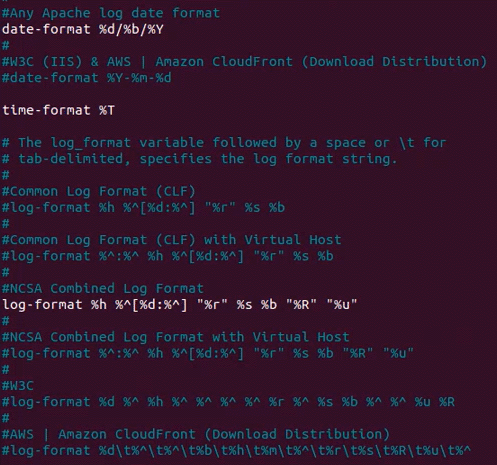
\includegraphics[width=256pt]{img/goaccess-conf.png}
        \caption{Content of \texttt{/etc/goaccess.conf} after modifications}
        \label{fig:goaccess-conf}
    \end{figure}
    
    To analyze local log files using \lstinline{goaccess}, execute:
    
    \termlbl{Server's Console}
    \lstsetterm
    \begin{lstlisting}
	goaccess -a > /var/www/html/report.html
    \end{lstlisting}
    
    To view the report of the \lstinline{goaccess}, start \textit{Mozilla Firefox} on the \textit{client} and navigate to this URL:
    
    \guilbl{\textit{gui}'s web browser}
    \lstsetgui
    \begin{lstlisting}
	https://128.238.66.100/report.html
    \end{lstlisting}
    
    Examine the web statistics displayed in the browser. Also click on the side panel to see other sections.

    \begin{report}
        \item List the most frequently visited pages at the local Apache server during the most recent month, respectively.
    
        \item List the web pages that have the most number of bytes transferred by the local during the most recent month, respectively.
    \end{report}

\newpage


% HELP: This section is confusing and unhelpful at the same time, which can be considered removed.
\section{** System Status}

Execute \lstinline{netstat -l} to display the listening sockets in server host.
    
    \termlbl{Server's Console}
    \lstsetterm
    \begin{lstlisting}
	netstat -l
    \end{lstlisting}

    Run these commands to see the system services info
    % HELP: This footnote was out of context:
    % \footnote{The old Linux OS service loaded in \path{/etc/init.d/} and \path{/etc/init/} directories}
    and their status:
    
    \begin{itemize}
        \item
        \termlbl{Server's Console}
        \lstsetterm
        \begin{lstlisting}
service --status-all
        \end{lstlisting}
        
       \textbf{Note: } The symbols shown to the left of each service name indicates its status:
        
        \begin{description}
        \item \lstinline{[+]} : Running
        \item \lstinline{[-]} : Stopped
        \item \lstinline{[?]} : Unknown
        \end{description}
        
        \item
        \termlbl{Server's Console} 
        \lstsetterm
        \begin{lstlisting}
	systemctl list-units --type=service --state=running
        \end{lstlisting}
    \textbf{Note: }This command may not be available on \lstinline{docker} \texttt{term} nodes.
        
        \item
        \termlbl{Server's Console} 
        \lstsetterm
        \begin{lstlisting}
	systemctl list-unit-files --type=service --state=enabled
        \end{lstlisting}
    \end{itemize}
    \textbf{Note: }This command may not be available on \lstinline{docker} \texttt{term} nodes.
    Save their output for the lab report.
    
    \begin{report}
        \item Are the \lstinline{rlogin}, \lstinline{ssh} and \lstinline{apache2} services
%        enabled and    % HELP: cannot check enabled status using the first command
        running on the \textit{server}?
    \end{report}

\end{document}
